% \documentclass[aspectratio=169]{beamer} % 16:9
\documentclass{beamer}
\usepackage{ctex, hyperref}
\usepackage[T1]{fontenc}
\graphicspath{{pic/}}

% other packages
\usepackage{latexsym, amsmath, xcolor, multicol,booktabs, calligra}
\usepackage{graphicx, pstricks, listings, stackengine}

\author[Sunbowen Lee]{李孙博闻}
\title[Graph neural network]{图神经网络的温和入门}
% \subtitle{图神经网络介绍}
\institute{武汉科技大学 \\ 理学院 \\ 冶金工业过程系统科学湖北省重点实验室}
\date{\today}
\usepackage{wust}

% 定义颜色
\def\cmd#1{\texttt{\color{red}\footnotesize $\backslash$#1}}
\def\env#1{\texttt{\color{blue}\footnotesize #1}}
\definecolor{deepblue}{rgb}{0,0,0.5}
\definecolor{deepred}{rgb}{0.6,0,0}
\definecolor{deepgreen}{rgb}{0.05, 0.44, 0.29}  % 青山绿
\definecolor{lightblue}{rgb}{0.63, 0.80, 0.86}  % 沁湖蓝

\lstset{
    basicstyle=\ttfamily\small,
    keywordstyle=\bfseries\color{deepblue},
    emphstyle=\ttfamily\color{deepred},    % Custom highlighting style
    stringstyle=\color{deepgreen},
    numbers=left,
    numberstyle=\small\color{halfgray},
    rulesepcolor=\color{red!20!green!20!blue!20},
    frame=shadowbox,
}


\begin{document}

\
\begin{frame}
    \titlepage
    \begin{figure}[htpb]
        \centering
        \vspace{-0.7cm}
        
\includegraphics[width=0.45\linewidth]{wust.png}
    \end{figure}
\end{frame}

\begin{frame}{目录}
    % \begin{multicols}{1}
        \tableofcontents[sectionstyle=show,subsectionstyle=hide]
    % \end{multicols}
\end{frame}


\section{图结构基础}

% \begin{itemize} % [<+-| alert@+>]

\begin{frame}{Vertex, Edge and Global}
    \begin{figure}
        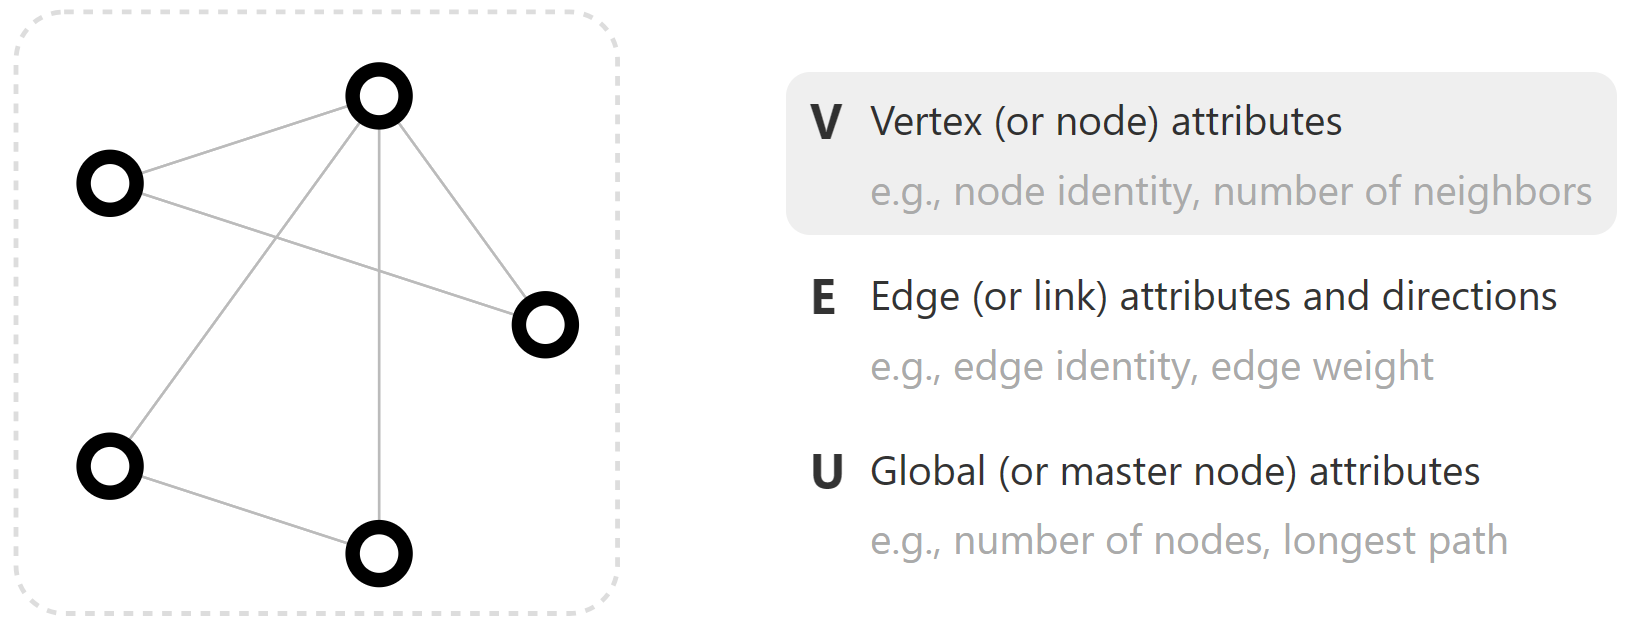
\includegraphics[width=\textwidth]{vertex.png}
    \end{figure}
\end{frame}

\begin{frame}{Vertex, Edge and Global}
    \begin{figure}
        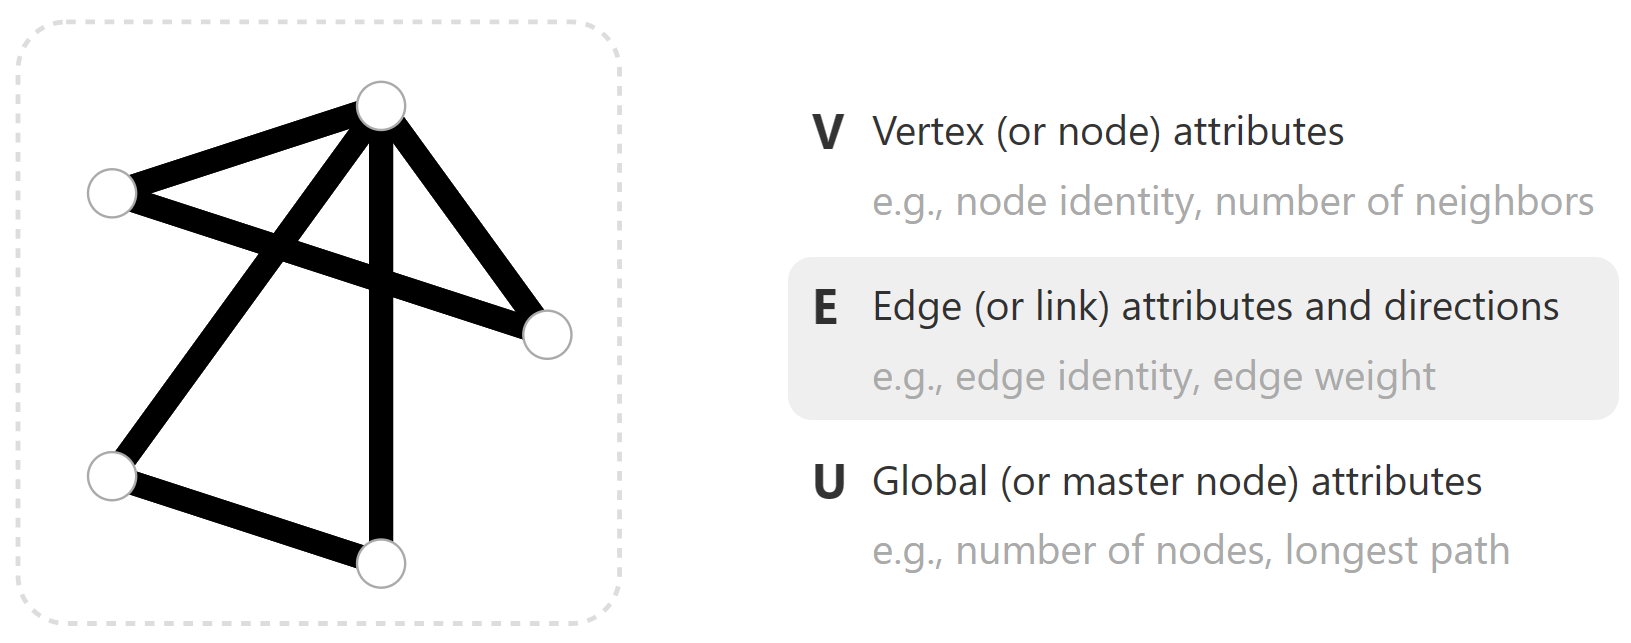
\includegraphics[width=\textwidth]{edge.png}
    \end{figure}
\end{frame}

\begin{frame}{Vertex, Edge and Global}
    \begin{figure}
        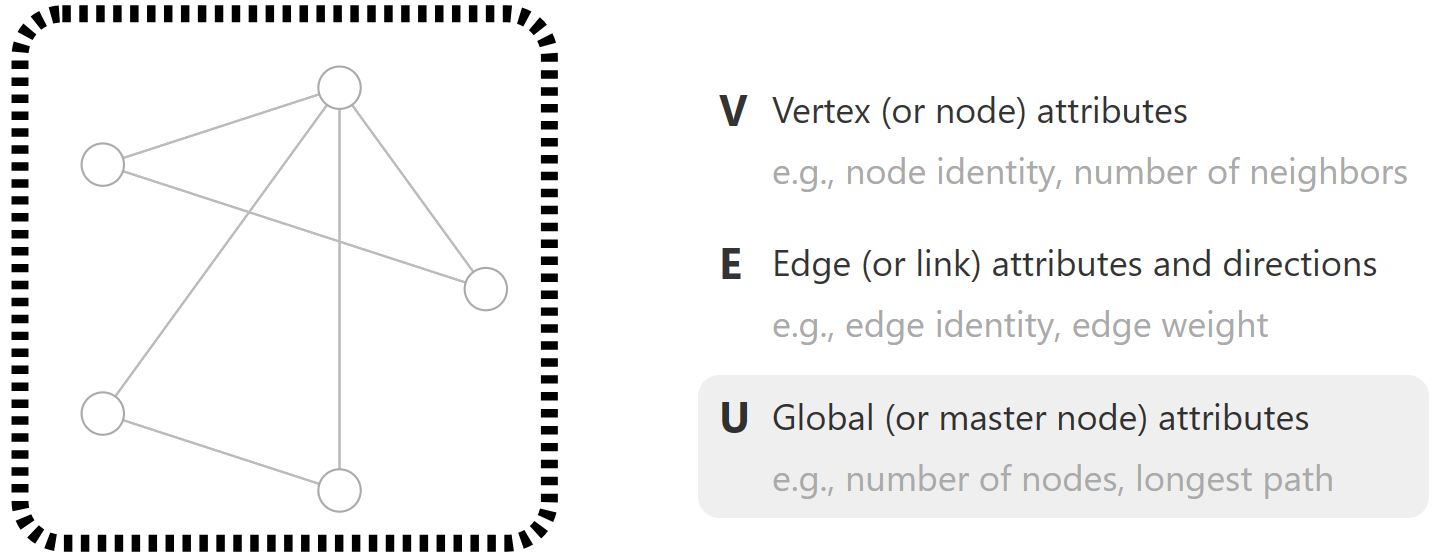
\includegraphics[width=\textwidth]{global.png}
    \end{figure}
    Note that letter U represents to global
\end{frame}

\begin{frame}{Vertex, Edge and Global}
    \begin{figure}
        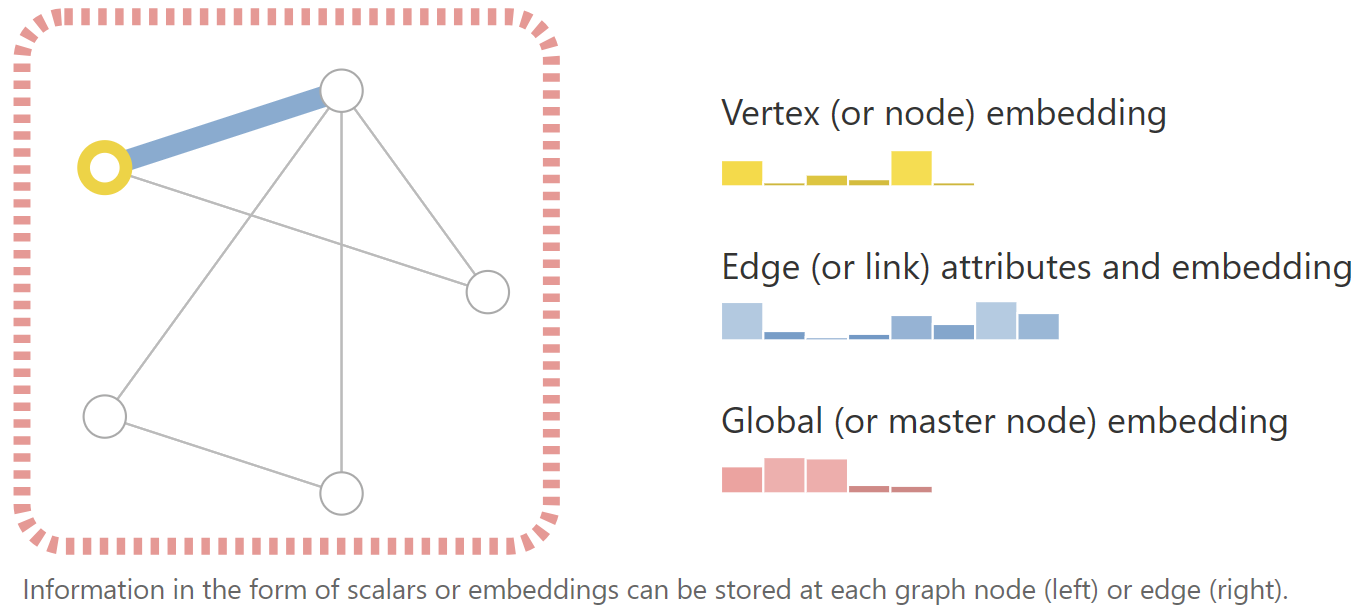
\includegraphics[width=\textwidth]{graph.png}
    \end{figure}
    Elements of graph can store embedding vectors.
\end{frame}

\section{图结构案例}

\subsection{空手道俱乐部}

\begin{frame}

\end{frame}


<<<<<<< HEAD
\section{图的任务}
=======
\section{图任务}
>>>>>>> 73e5e60bd7aa3bf41ce4f656998c52b51f00c582

\begin{frame}

\end{frame}

\section{图的构建}

\begin{frame}

\end{frame}

\section{图神经网络}

\begin{frame}

\end{frame}

\section{参考文献}

\begin{frame}[allowframebreaks]
    \bibliography{ref}
    \bibliographystyle{alpha}
    % 如果参考文献太多的话,可以像下面这样调整字体:
    % \tiny\bibliographystyle{alpha}
\end{frame}

\begin{frame}
    \begin{center}
        {\Huge\calligra Thanks!}
    \end{center}
\end{frame}

\end{document}